


\chapter{Introduction}

\section{Visualizing Structure in Datasets}

In the modern world data is collected on a daily basis. When collectinng information about patients, companies, countries (\ie datapoints) policy makers have to deal with complex and high dimensional feature spaces. Most of these datasets however contain low dimensional structure, which is really of interest. Before she starts searching for information the researcher therefore embeds the data in a visualizable space, often the 2D-plane. This procedure not only helps to get an overview of the dataset but is also able to find clusters of points, which share certain features. To main goal of data visualization is therefore to embed datasets in low dimensional spaces without loosing too much structure, a task which is not optimally solvable but subject to different trade-offs and design decisions.  One particular method that we will use throughout this thesis, is called t-Stochastic Neighbor Embedding (t-SNE) (see section \ref{tSNE}.

\subsection{Motivational example}

To illustrate the effects of data visualization let's have a look at the election of Baden-Würtemberg in March 2021. Eventually an election is boiled down to a six dimensional vector \footnote{for simplicity we consider here (and in later analysis) only the six major parties CDU, SPD, DIE GRÜNEN, AfD, FDP and DIE LINKE} containing the final results, however these results may vary among voting districts. The complete election dataset is therefore a six-dimensional space where the 72 voting districts are single points. In Figure \ref{intro:bawu} we used t-SNE to embed these voting districts onto the 2D plane.

\begin{figure}[h]
	\centering
	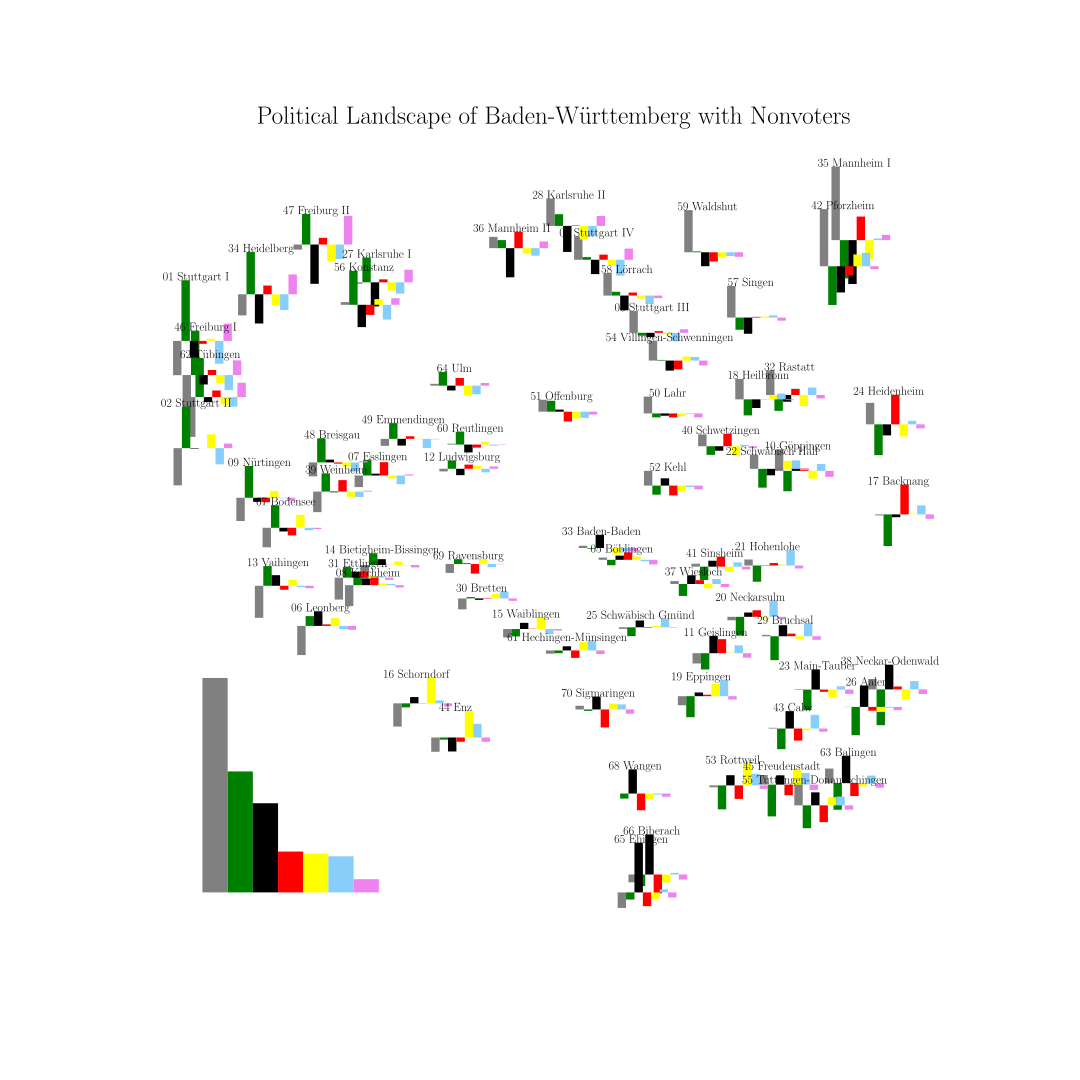
\includegraphics[width=\textwidth]{assets/infoBW2021_NWTrue.pdf}
	\caption{Baden-Würtemberg election 2021}
	\label{intro:bawu}
\end{figure}

We can see here the different voting district with their corresponding election result. Similar district should be embedded in a similar region. Since the full data ist seven dimensional (six major parties plus onvoter share) this task is impossible to solve accuratley. The t-SNE algorithm puts emphasis on close point in the high dimensional space. Thus, neighbors stay neighbors in the embedding. 

\subsection{Design choices}

NOte, that the minimizatoin problem is not comvex, thus it has mutltipke local minimal. With different initialization the algorithm find different embeddings. 


\section{Hierarchical Data}

While most datasets contain vector-shaped datapoints, often there are two or more levels in which these datapoints are arranged. As an example one can think of participants of a study in diofferent regions of the world. When we now want to visualize similarieties and difference of countries, we no longer embed vectors but probability distributions from which we have as samples the participants of the respective nationality. Table  

\begin{table}[h]
\begin{tabular}{llllll}
\multicolumn{1}{l|}{}                     & \textbf{AGR} & \textbf{CSN} & \textbf{EST} & \textbf{EXT} & \textbf{OPN} \\ \hline
\multicolumn{1}{l|}{United Arab Emirates} & 4.8          & 4.6          & 1.9          & 1.8          & 4.7          \\
\multicolumn{1}{l|}{United Arab Emirates} & 2.1          & 4.3          & 2.5          & 1.5          & 4.7          \\
\multicolumn{1}{l|}{United Arab Emirates} & 4.5          & 2.1          & 3.2          & 1.9          & 3.5          \\
\multicolumn{1}{l|}{United Arab Emirates} & 3.9          & 2.4          & 2.0          & 1.4          & 3.9          \\
\multicolumn{1}{l|}{United Arab Emirates} & 3.9          & 2.4          & 1.6          & 3.0          & 4.6          \\
\multicolumn{1}{l|}{...}                  & ...          & ...          & ...          & ...          & ...          \\
\multicolumn{1}{l|}{Zimbabwe}             & 3.5          & 4.6          & 2.4          & 2.1          & 4.9          \\
\multicolumn{1}{l|}{Zimbabwe}             & 3.1          & 3.4          & 2.0          & 2.8          & 4.7          \\
\multicolumn{1}{l|}{Zimbabwe}             & 2.9          & 2.2          & 2.9          & 4.8          & 4.4          \\
\multicolumn{1}{l|}{Zimbabwe}             & 4.6          & 3.6          & 1.9          & 1.7          & 4.6          \\
\multicolumn{1}{l|}{Zimbabwe}             & 4.3          & 3.5          & 3.5          & 1.5          & 4.6          \\
{[}219584 rows x 5 columns{]}             &              &              &              &              &              
\end{tabular}
\caption{Overview of the BIG5 Personality dataset}
\label{tab:big5}
\end{table}

We can see here the design of the data, each country has multiple participants of whcih each correpsonds to a 5 dimnesional vector of his personality \footnote{actually the datasets contains up to 50 features (ten per trait) which I averaged for simplicity. \ref{intro:big5corr} justifies why one can do that}.

\subsection{Mean embedding}

The most natural choice to embed a hierarchical dataset is just to collapse the probabilty distribution into the mean. Figure \ref{intro:big5} shows this 

\begin{figure}[h]
	\centering
	\includegraphics[width=\textwidth]{BIG5/EmbeddingContinents.pdf}
	\caption{Big 5 Personality Traits}
	\label{intro:big5}
\end{figure}


\subsection{Including covariance}

While for some datasets it might be sufficient to ignore other moments by averaging the samples into the mean, this thesis will explore how much information is lost in this way, and we will propose a method that included the Covariance and later even the full information by using the Wasserstein metric of distributions. As an indication of why this might be necessary, let us look at Figure


\begin{figure}[h]
	\centering
	\includegraphics[width=\textwidth]{BIG5/Overview.pdf}
	\caption{Correlation of Features}
	\label{intro:big5corr}
\end{figure}


\section{Outline}

The goal of this thesis is to show that in combination of the previous two section it is helkpful to include the Structure of Covariance and other higher moments) into the embedding or clustering of hierarchical data.  I will analyze two well known datasets, the German Federal Election and the European Values Study, to show the benefits and downsides of our method. IN the next chapter however, I will give an overview of the relevant mathematical background and explain various algorithm and their design choices. In additon I propose a technique to compute the Exact Wasserstein distance, which is known to be intractable for higher dimensions. 